\let\negmedspace\undefined
\let\negthickspace\undefined
\documentclass[journal]{IEEEtran}
\usepackage[a5paper, margin=10mm, onecolumn]{geometry}
\usepackage{lmodern} % Ensure lmodern is loaded for pdflatex
\usepackage{tfrupee} % Include tfrupee package

\setlength{\headheight}{1cm} % Set the height of the header box
\setlength{\headsep}{0mm}     % Set the distance between the header box and the top of the text

\usepackage{gvv-book}
\usepackage{gvv}
\usepackage{cite}
\usepackage{amsmath,amssymb,amsfonts,amsthm}
\usepackage{algorithmic}
\usepackage{graphicx}
\usepackage{textcomp}
\usepackage{xcolor}
\usepackage{txfonts}
\usepackage{listings}
\usepackage{enumitem}
\usepackage{mathtools}
\usepackage{gensymb}
\usepackage{comment}
\usepackage[breaklinks=true]{hyperref}
\usepackage{tkz-euclide} 
\usepackage{listings}
\usepackage{gvv}                                        
\def\inputGnumericTable{}                                 
\usepackage[latin1]{inputenc}                                
\usepackage{color}                                            
\usepackage{array}                                            
\usepackage{longtable}                                       
\usepackage{calc}                                             
\usepackage{multirow}                                         
\usepackage{hhline}                                           
\usepackage{ifthen}                                           
\usepackage{lscape}
\begin{document}

\bibliographystyle{IEEEtran}
\vspace{3cm}

\title{11.16.3.19}
\author{EE24BTECH11034 - K Teja Vardhan}
% \maketitle
% \newpage
% \bigskip
{\let\newpage\relax\maketitle}
\textbf{Question:\\}
In an entrance test graded on the basis of two examinations, the probability of a randomly chosen student passing the first examination is 0.8, and the probability of passing the second examination is 0.7. The probability of passing at least one of them is 0.95. What is the probability of passing both?\\
\solution\\


P(A): Probability of passing the first exam.\\
P(B): Probability of passing the second exam.\\
P(A+B): Probability of passing at least one exam.\\
p(AB) : probability of passing both\\
\begin{align}
	\Pr\brak{A} &= 0.8\\
	\Pr\brak{B} &= 0.7\\
	\Pr\brak{A \cup B} &= 0.95
\end{align}
Find \(\Pr\brak{A \cap B}\)\\


\textbf{Theoretical Solution:\\}
For 2 Boolean variables \(A\) and \(B\), the axioms of Boolean Algebra are defined as:
\begin{align}
	A + A^\prime &= 1\\
	A + A &= A\\
	AB &= BA\\
	A + B &= B + A\\
	AA^\prime &= 0\\
	\Pr\brak{1} &= 1\\
	\Pr\brak{A + B} &= \Pr\brak{A} + \Pr\brak{B}, \text{ if } \Pr\brak{AB} = 0
\end{align}
Using these axioms, we will try to prove that
\begin{align}
	\Pr\brak{A + B} = \Pr\brak{A} + \Pr\brak{B} - \Pr\brak{AB}
\end{align}
We will start by representing \(A\) and \(B\) as:
\begin{align}
	A &= AB + AB^\prime\\
	B &= AB + A^\prime B\\
	\Pr\brak{A} &= \Pr\brak{AB} + \Pr\brak{AB^\prime}\\
	\Pr\brak{B} &= \Pr\brak{AB} + \Pr\brak{A^\prime B}
\end{align}
On adding \(\brak{12}\) and \(\brak{13}\),
\begin{align}
	A + B &= AB + AB + AB^\prime + A^\prime B\\
	A + B &= AB + AB^\prime + A^\prime B\\
	\Pr\brak{A + B} &= \Pr\brak{AB + AB^\prime + A^\prime B}\\
	\Pr\brak{A + B} &= \Pr\brak{AB} + \Pr\brak{AB^\prime} + \Pr\brak{A^\prime B}\\
	\Pr\brak{A + B} &= \Pr\brak{AB} + \Pr\brak{A} - \Pr\brak{AB} + \Pr\brak{B} - \Pr\brak{AB}\\
	\implies \Pr\brak{A + B} &= \Pr\brak{A} + \Pr\brak{B} - \Pr\brak{AB}
\end{align}
Using the given values of \(\Pr\brak{A}\), \(\Pr\brak{B}\), and \(\Pr\brak{A \cup B}\),
\begin{align}
	\Pr\brak{A \cup B} &= \Pr\brak{A} + \Pr\brak{B} - \Pr\brak{A \cap B}\\
	0.95 &= 0.8 + 0.7 - \Pr\brak{A \cap B}\\
	\Pr\brak{A \cap B} &= 0.8 + 0.7 - 0.95\\
	\Pr\brak{A \cap B} &= 0.55
\end{align}
Therefore, the value of \(\Pr\brak{A \cap B}\) is \(0.55\).\\\\
\textbf{Simulated Solution:\\}
Let \(X_1\) be an indicator random variable of the event \(A\).\\
\(X_1\) is defined as:
\begin{align}
	X_1 =
	\begin{cases}
		1 ,& A\\
		0 ,& A^\prime\\
	\end{cases}
\end{align}
Let \(X_2\) be the indicator random variable of the event \(B\).\\
\(X_2\) is defined as:
\begin{align}
	X_2 =
	\begin{cases}
		1 ,& B\\
		0 ,& B^\prime\\
	\end{cases}
\end{align}
Let \(X_3\) be the indicator random variable of the event \(AB\).\\
\(X_3\) is defined as:
\begin{align}
	X_3 =
	\begin{cases}
		1 ,& AB\\
		0 ,& \brak{AB}^\prime\\
	\end{cases}
\end{align}
The PMF of the random variable \(X_1\) is:
\begin{align}
	p_{X_1}\brak{n} =
	\begin{cases}
		p_1 ,& n = 1\\
		1 - p_1 ,& n = 0
	\end{cases}
\end{align}
The PMF of the random variable \(X_2\) is:
\begin{align}
	p_{X_2}\brak{n} =
	\begin{cases}
		p_2 ,& n = 1\\
		1 - p_2 ,& n = 0
	\end{cases}
\end{align}
The PMF of the random variable \(X_3\) is:
\begin{align}
	p_{X_3}\brak{n} =
	\begin{cases}
		p_3 ,& n = 1\\
		1 - p_3 ,& n = 0
	\end{cases}
\end{align}
where,
\begin{align}
	p_1 &= 0.8\\
	p_2 &= 0.7\\
	p_3 &= 0.55\\
\end{align}
Let \(Y\) be the random variable which is defined as follows:
\begin{align}
	Y = X_1 + X_2 - X_3
\end{align}
But we know that \(X_3\) can never be \(0\) when \(X_1\) and \(X_2\) are \(1\) and vice versa.\\
So, \(Y\) is another Indicator Random variable whose PMF is defined as:
\begin{align}
	p_{Y}\brak{n} =
	\begin{cases}
		p ,& n = 1\\
		1 - p ,& n = 0
	\end{cases}
\end{align}
From \(\brak{34}\),
\begin{align}
	E\brak{Y} &= E\brak{X_1 + X_2 - X_3}\\
	E\brak{Y} &= E\brak{X_1} + E\brak{X_2} - E\brak{X_3}\\
	1.\brak{p} + 0.\brak{1 - p} &= 1.\brak{p_1} + 0.\brak{1 - p_1} + 1.\brak{p_2} + 0.\brak{1 - p_2} - 1.\brak{p_3} - 0.\brak{1 - p_3}\\
	p &= p_1 + p_2 - p_3
\end{align}
Through our definition, we know that,
\begin{align}
	\Pr\brak{A} = p_1\\
	\Pr\brak{B} = p_2\\
	\Pr\brak{AB} = p_3
\end{align}
Therefore, by comparison of the axiom
\begin{align}
	\Pr\brak{A + B} = \Pr\brak{A} + \Pr\brak{B} - \Pr\brak{AB}
\end{align}
and the equation \(\brak{39}\),
\begin{align}
	p &= \Pr\brak{A + B}\\
	\Pr\brak{A + B} &= 0.8 + 0.7 - 0.55\\
	\implies \Pr\brak{A + B} &= 0.95
\end{align}

\pagebreak
Below is the plot for the simulation of the probabilities, where the grey stems represent the theoretical probabilities and the coloured stems represent the simulated ones.\\
Through observation in the last stem, we have proved through the code that
\begin{align}
	\Pr\brak{A + B} = \Pr\brak{A} + \Pr\brak{B} - \Pr\brak{AB}
\end{align}

\begin{figure}[h!]
	\centering
	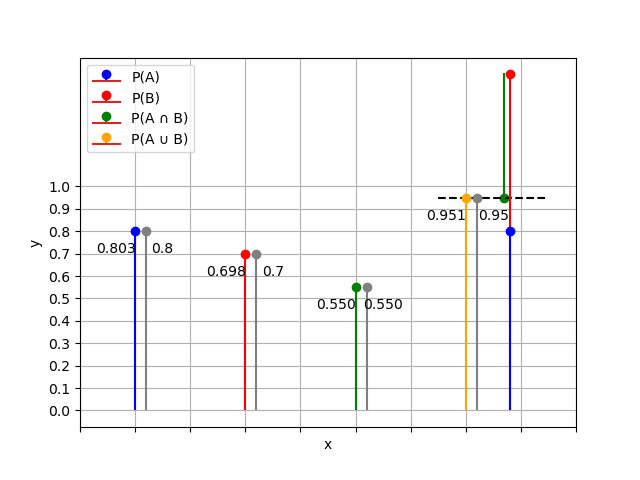
\includegraphics[width=1\columnwidth]{figs/simulated.png}
	\caption{Plot of the probabilities}
	\label{stemplot}
\end{figure}

\end{document}
